\chapter{Ergänzungen zur Simulation von Gold-PVD}

\begin{figure}[!h]
  \captionsetup[subfigure]{singlelinecheck=false}
  \def\subfigwidth{0.49\textwidth}

  \begin{subfigure}[t]{\subfigwidth}
    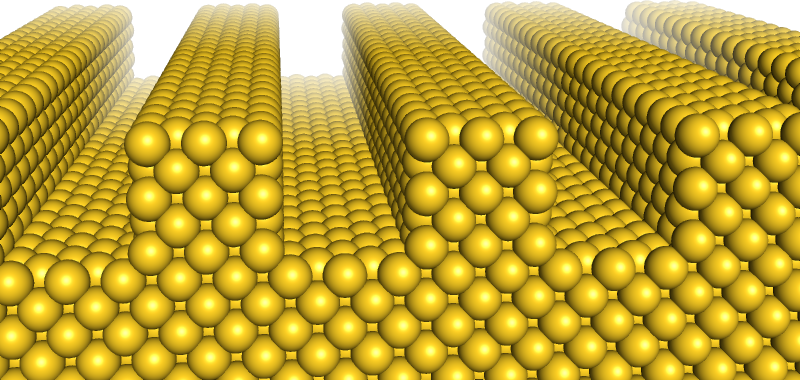
\includegraphics[width=\textwidth]{Au_fin_01}
    \subcaption{Substrat mit Gold-Lamellen}
    \label{fig:goldnanostructures-fins}
  \end{subfigure}
  \hfill
  \begin{subfigure}[t]{\subfigwidth}
    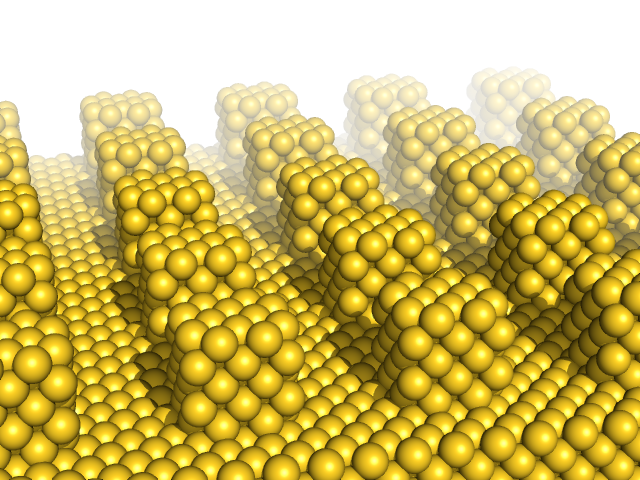
\includegraphics[width=\textwidth]{Au_pillars_1}
    \subcaption{Substrat mit Gold-Säulen}
    \label{fig:goldnanostructures-columns}
  \end{subfigure}

  \caption{Substrate mit einer Strukturbreite von \SI{1}{\nano\meter} zur Prüfung der Robustheit}
  \label{fig:goldnanostructures}

\end{figure}

\begin{figure}[!h]
  \captionsetup[subfigure]{singlelinecheck=false}
  \def\subfigwidth{0.49\textwidth}

  \begin{subfigure}[t]{\subfigwidth}
    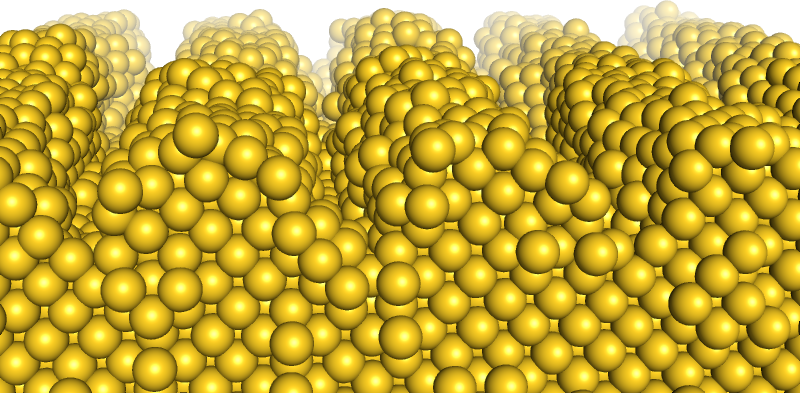
\includegraphics[width=\textwidth]{Au_fin_03}
    \subcaption{Substrat mit Gold-Lamellen}
    \label{fig:goldnanostructures-fins}
  \end{subfigure}
  \hfill
  \begin{subfigure}[t]{\subfigwidth}
    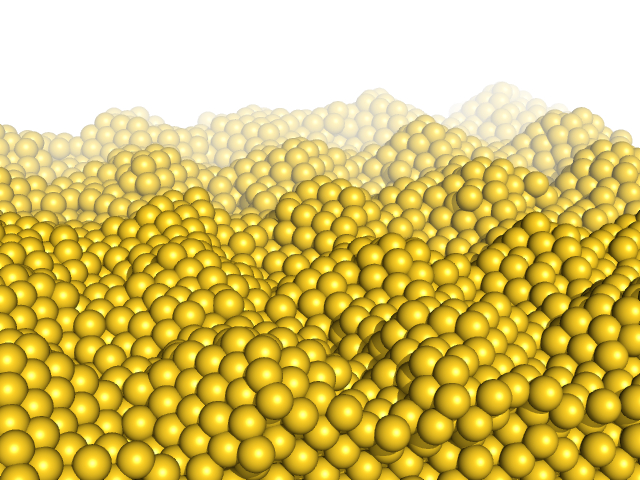
\includegraphics[width=\textwidth]{Au_pillars_3}
    \subcaption{Substrat mit Gold-Säulen}
    \label{fig:goldnanostructures-columns}
  \end{subfigure}

  \caption{Oberfläche nach zwei Parsivald-Zyklen ($\approx \SI{2}{\angstrom}$ Schichtwachstum)}
  \label{fig:goldnanostructures}

\end{figure}

\begin{figure}[!h]
  \captionsetup[subfigure]{singlelinecheck=false}
  \def\subfigwidth{0.49\textwidth}

  \begin{subfigure}[t]{\subfigwidth}
    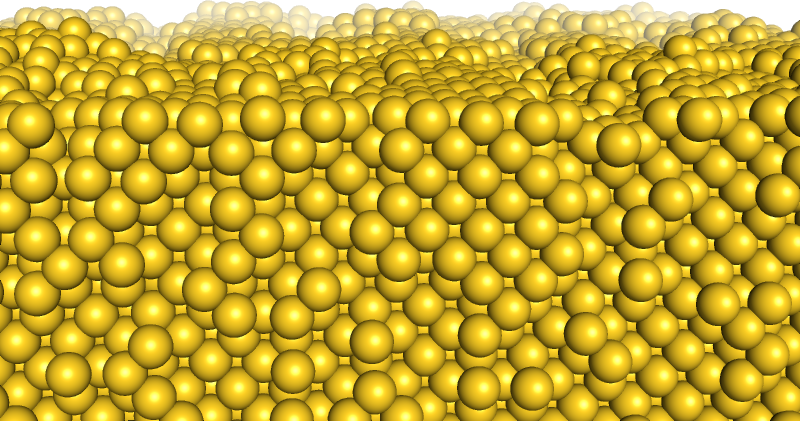
\includegraphics[width=\textwidth]{Au_fin_10}
    \subcaption{Substrat mit Gold-Lamellen}
    \label{fig:goldnanostructures-fins}
  \end{subfigure}
  \hfill
  \begin{subfigure}[t]{\subfigwidth}
    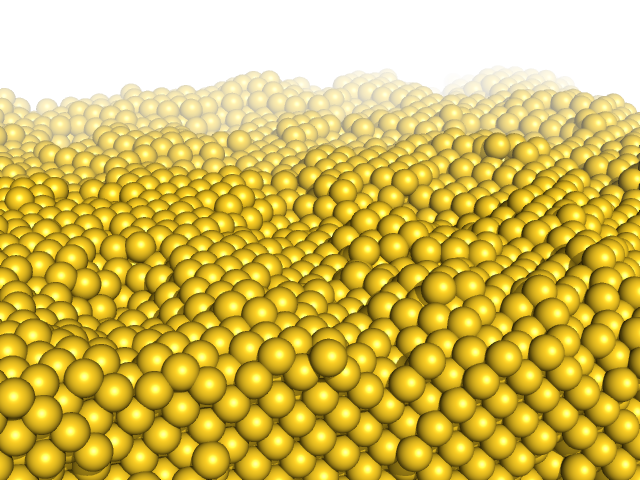
\includegraphics[width=\textwidth]{Au_pillars_8}
    \subcaption{Substrat mit Gold-Säulen}
    \label{fig:goldnanostructures-columns}
  \end{subfigure}

  \caption{Oberfläche nach acht Parsivald-Zyklen ($\approx \SI{2}{\angstrom}$ Schichtwachstum)}
  \label{fig:goldnanostructures}

\end{figure}
